\documentclass{standalone}
\usepackage{tikz}
\usetikzlibrary{matrix, fit}

\begin{document}
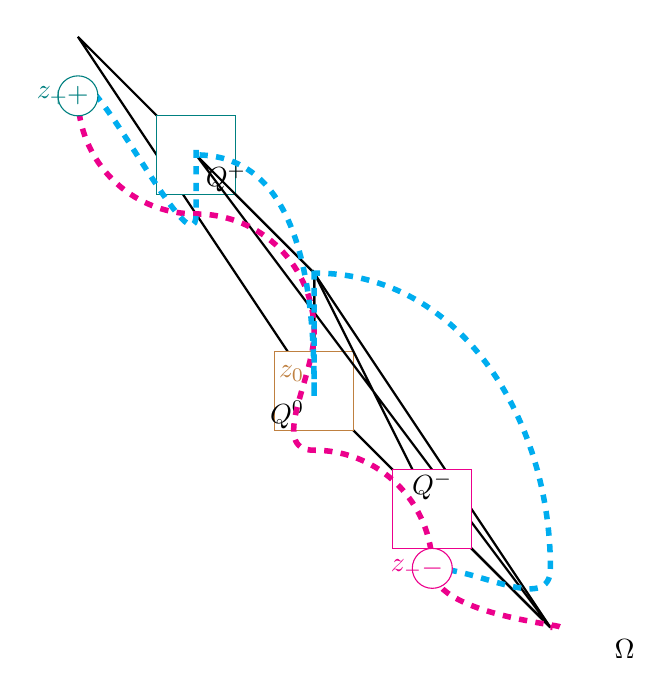
\begin{tikzpicture}[scale=1.5]
    % Define coordinates for the points
    \coordinate (Q1) at (-2, 4);
    \coordinate (Q2) at (-1, 3);
    \coordinate (Q3) at (0, 2);
    \coordinate (Q4) at (0, 1);
    \coordinate (Q5) at (1, 0);
    \coordinate (Q6) at (2, -1);

    % Define the points for the curves
    \coordinate (Z1) at (-2, 3.5);
    \coordinate (Z2) at (-1, 2.5);
    \coordinate (Z3) at (0, 1.5);
    \coordinate (Z4) at (0, 0.5);
    \coordinate (Z5) at (1, -0.5);
    \coordinate (Z6) at (2, -0.5);

    % Draw the rectangles representing regions Q^+, Q^0, and Q^-
    \draw[thick] (Q1) -- (Q2) -- (Q3) -- (Q4) -- cycle;
    \node[draw=teal, fill=white, inner sep=0pt, minimum size=1cm] at (Q2) {};
    \node[below right] at (Q2) {$Q^+$};

    \draw[thick] (Q5) -- (Q6) -- (Q3) -- (Q4) -- cycle;
    \node[draw=brown, fill=white, inner sep=0pt, minimum size=1cm] at (Q4) {};
    \node[below left] at (Q4) {$Q^0$};

    \draw[thick] (Q6) -- (Q5) -- (Q3) -- (Q2) -- cycle;
    \node[draw=magenta, fill=white, inner sep=0pt, minimum size=1cm] at (Q5) {};
    \node[above] at (Q5) {$Q^-$};

    % Draw the dashed curves Γ_
    \draw[dashed, magenta, line width=2pt] (Z1) to[out=-90,in=180] (Z2) to[out=0,in=90] (Z3) to[out=-90,in=180] (Z4) to[out=0,in=90] (Z5) to[out=-90,in=0] (Q6);

    % Draw the dashed curves Γ+
    \draw[dashed, cyan, line width=2pt] (Z5) to[out=0,in=-90] (Z6) to[out=90,in=0] (Q3) to[out=90,in=-90] (Q4) to[out=90,in=0] (Q2) to[out=90,in=90] (Z2) to[out=-90,in=90] (Z1);

    % Mark the points z_+ and z_- with a plus sign
    \node[circle, draw=teal, fill=white, inner sep=1.5pt] at (Z1) {\textcolor{teal}{$+$}};
    \node[circle, draw=magenta, fill=white, inner sep=1.5pt] at (Z5) {\textcolor{magenta}{$-$}};

    % Add labels for z_+ and z_-
    \node[anchor=east] at (Z1) [color=teal] {$z_+$};
    \node[anchor=east] at (Z5) [color=magenta] {$z_-$};

    % Add the label for the region Q^0
    \node[anchor=south east] at (Q4) [color=brown] {$z_0$};

    % Add the label for Ω
    \node[below right] at (current bounding box.south east) {$\Omega$};
\end{tikzpicture}
\end{document}